%\documentclass[compress,xcolor=table]{beamer}
\usepackage{etex}
%\documentclass{article}
%\usepackage{beamerarticle}
%\usepackage{pstricks,pst-node} % PSTricks package
\usepackage{tikz}
\usetikzlibrary{patterns,positioning,fit,arrows,matrix,calc,shapes.geometric,shapes.multipart,decorations.pathreplacing}
%\usepackage[turkish]{babel}
\usepackage[utf8]{inputenc}
\usepackage{listings}
\usepackage{multicol}
%\includeonlyframes{current}

\mode<article>
{
  \usepackage{fullpage}
  \usepackage{pgf}
  \usepackage{hyperref}
}

\mode<presentation>
{
  \usetheme{metuceng}

  %\setbeamercovered{transparent}
}


\title{Programming Languages}
\subtitle{Control Flow}
\author{Onur Tolga Şehitoğlu}
\institute[METU]{Computer Engineering}
\subject{Control Flow}
\date{}
	\titlegraphic{\insertmetutitle\insertlicense}


\def\circtxt#1{$\mathalpha \bigcirc \mkern-13mu \mathtt #1$}
\def\smiley{\textcircled{\scriptsize $\mkern3mu\ddot{\ } \mkern-15mu \smallsmile$}}

\begin{document}

\lstset{language=C,
        basicstyle=\scriptsize\ttfamily,
        keywordstyle=\color{blue!50!black}\bfseries,
        identifierstyle=\color{blue!60!green}\sffamily,
        stringstyle=\color{red!70!green}\ttfamily,
	commentstyle=\color{blue!30!white}\itshape,
        showstringspaces=true}
\setbeamercolor{hexample}{bg=green!5!white,fg=black}%
\setbeamercolor{cexample}{bg=blue!5!white,fg=black}%
\setbeamercolor{pexample}{bg=orange!5!white,fg=black}%
\setbeamercolor{oexample}{bg=violet!5!white,fg=black}%

 \frame[plain]{\maketitle}
 \begin{frame}
 \frametitle{Outline}
 \begin{multicols}{2}
 \small
 \tableofcontents
 \end{multicols}
 \end{frame}
\section{Control Flow}
\begin{frame}
\frametitle{Control Flow}
\begin{itemize}
\item Usual control flow: a command followed by the other. Executed in sequence.
\structure{single entrance - single exit}
\item Commands to change control flow and transfer execution to another point: 
\structure{sequencers}
\begin{itemize}
\item Jumps
\item Escapes
\item Exceptions
\end{itemize}
\end{itemize}
\end{frame}

\newcommand{\R}[2]{\tikz [remember picture,overlay] \node (#1) {#2};}

\defverbatim[colored]\codejump{
\begin{lstlisting}[language={C},escapechar=\#]
#\R{l1}{}#L1:  x++;
     if (x>10) goto L2#\R{gl2}{}#;
     j++;
     for (i=0;i<j;j++) {
         x=x*2;
#\R{l2}{}#L2:      if (x>1000) goto L3#\R{gl3}{}#;
         else goto L1#\R{gl1}{}#;
     }
#\R{l3}{}#L3:  printf("out\n");
\end{lstlisting}}
\section{Jumps}
\begin{frame}
\frametitle{Jumps}
\begin{itemize}
\item Jumps transfer control to a point in the code. The destination is marked with
\structure{labels}
\item When jumps to arbitrary positions are possible...:
\begin{beamercolorbox}{cexample}
\codejump
\end{beamercolorbox}
\only<2->{\begin{tikzpicture} [thick,remember picture,overlay,rounded corners=3pt]
\draw [green,->] (gl1) -- +(0,2.5) -| (l1);
\draw [violet,->] (gl2) -- +(0,-0.3) -|  (l2);
\draw [red,->] (gl3) -- +(0,-1.5) -| (l3);
\end{tikzpicture}}
%\ncbar[linecolor=green,angleA=90,angleB=90,nodesep=2pt,linearc=.3,arm=15pt]{->}{gl1}{l1} 
%\ncbar[linecolor=magenta,angleA=90,angleB=90,nodesep=2pt,linearc=.3,arm=15pt]{->}{gl2}{l2} 
%\ncbar[linecolor=red,angleA=-90,angleB=-90,nodesep=2pt,linearc=.3,arm=15pt]{->}{gl3}{l3} }
\item Called \structure{spaghetti coding}
\end{itemize}
\end{frame}

\defverbatim[colored]\codejumpblock{
\begin{lstlisting}[language={C},escapechar=\#]
L1: ....
    goto L2;        #\color{violet}\circtxt{1}#
    ....
    for (i=0;i<10;i++) {
        int x=t;
L2:     ....
        goto L1;    #\color{violet}\circtxt{2}#
	...
	goto L2:    #\color{violet}\circtxt{3}#
    }
\end{lstlisting}}
\begin{frame}
\small
\begin{itemize}
\item Unrestricted jumps $\Rightarrow$ spaghetti coding.
\item GCC extension allows storing labels in variables. Would you like to debug that code? \smiley
\item Further problems. Which jumps have problems?:
\begin{beamercolorbox}{cexample}
\codejumpblock
\end{beamercolorbox}
\item Lifetime and values of local variables? Values of index variables?
\item C: Labels are local to enclosing block. No jumps allowed into the block.
Newer languages avoid jumps.
\item Single entrance multiple exit is still desirable.$\rightarrow$ escapes
\end{itemize}
\end{frame}

\section{Escapes}
\begin{frame}
\frametitle{Escapes}
\begin{itemize}
\item  Restricted jumps to out of textually enclosing block(s)
\item Depending on which enclosing block to jump out of:
\begin{itemize}
\item loop: \structure{break} sequencer.
\item loops: \structure{exit} sequencer.
\item function: \structure{return} sequencer.
\item program: \structure{halt} sequencer.
\end{itemize}
\end{itemize}
\end{frame}

\defverbatim[colored]\codejavaescapes{
\begin{lstlisting}[language={Java},escapechar=\#]
L1:  for (i=0;i<10;i++) {
        for (j=i;j<i;j++) {
	   if (...) break;
	   else if (...) continue;
	   else if (...) break L1;
	   else if (...) continue L1;
	   s+=i*j;
	}
     }
\end{lstlisting}}
\begin{frame}
\begin{itemize}
\item \structure{break sequencer} in C, C++, Java terminates the innermost
	enclosing loop block.
\item \structure{continue} in C, C++ stays in the same block but ends current iteration.
\item \structure{exit sequencer} in Ada or labeled \texttt{break} in Java can terminate
multiple levels of blocks by specifying labels. Java code:\\
\begin{beamercolorbox}{oexample}
\codejavaescapes
\end{beamercolorbox}
\end{itemize}
\end{frame}

\defverbatim[colored]\codejumpfunc{
\begin{lstlisting}[language={C},escapechar=\#]
int f(int n) {
    int a;

L1: if (n<0) goto L2;   #\color{violet}\circtxt{1}#
    else if (n=1) return 1;
    else return f(n-1)*n;
}
int main() {
    ...
    f(12);
L2: ....
    goto L1:             #\color{violet}\circtxt{2}#
    }
\end{lstlisting}}
\begin{frame}
\begin{itemize}
\item \structure{return sequencer} exist in most languages for terminating the innermost
function block.
\item \structure{halt sequencer} either provided by operating system or PL terminates the
program.
\item Consider jump inside of a block or jump out of a block for the function case:
\begin{beamercolorbox}{cexample}
\codejumpfunc
\end{beamercolorbox}
\end{itemize}
\end{frame}

\begin{frame}
\begin{itemize}
\item Jump out  of a function block, jump inside of a function block
\item Jumps update current instruction pointer. But what about environment, activation record 
    (run-time stack)? 
\item Possible only for one direction if stack position can be recovered. Called \structure{non-local jumps}\\
{\tiny 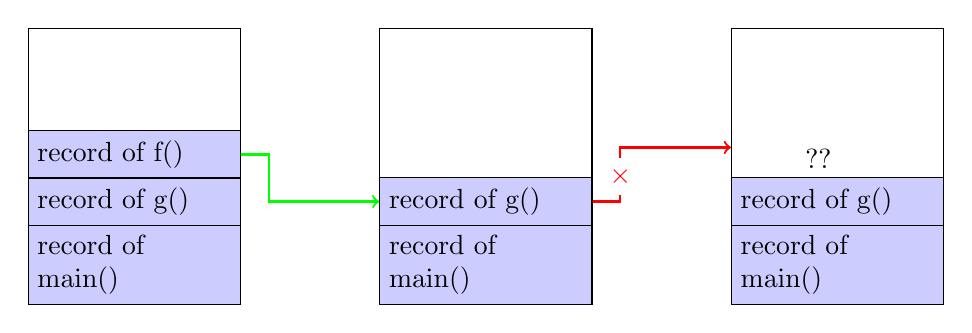
\begin{tikzpicture}
   [stack/.style={rectangle split, rectangle split parts=4,draw,
     text width=7em},
    scolor/.style={rectangle split part fill={white,blue!20!white,blue!20!white,blue!20!white}}]

\node [stack,scolor] (stk1) {
\nodepart{one} \rule{0pt}{3em}
\nodepart{two} record of f()
\nodepart{three} record of g()
\nodepart{four} record of main()
};
\node [stack,scolor,rectangle split parts=3, right=5em of stk1] (stk2) {
\nodepart{one} \rule{0pt}{4.7em}
\nodepart{two} record of g()
\nodepart{three} record of main()
};
\node [stack,scolor, rectangle split parts=3,right=5em of stk2] (stk3) {
\nodepart{one} \rule{0pt}{4.7em}\hspace*{2em} ??
\nodepart{two} record of g()
\nodepart{three} record of main()
};
\draw [->,green,thick] (stk1.two east) -- +(1em,0) |- (stk2.two west);
\draw [->,red,thick] (stk2.two east) -- +(1em,0) node [fill=white, yshift=.9em] {$\times$} |-  ($(stk3.one west) - (0,1.6em)$);
\end{tikzpicture}
}
\item Are non-local jumps useful? One of the uses: unexpected error occuring inside of many levels of recursion. Jump to
	the outer-most related caller function. \structure{Exceptions}
\end{itemize}
\end{frame}

\section{Exceptions}
\begin{frame}
\frametitle{Exceptions}
\begin{itemize}
\item Controlled jumps out of multiple levels of function calls to an outer control
	point (\texttt{handler} or \texttt{catch})
\item C does not have exceptions but non-local jumps possible via \texttt{setjmp()},
\texttt{longjmp()} library calls.
\item C++ and Java: \texttt{try \{...\} catch(...) \{...\}}
\item Each \texttt{try-catch} block introduces a non-local jump point. \texttt{try} block
	is executed and whenever a \texttt{throw {\em expr\/}} command is called in any functions
	called (even indirectly) inside \texttt{try}  block execution jumps to the
	\texttt{catch()} part.
\item \texttt{try-catch} blocks can be nested. Execution jumps to closes 
\texttt{catch} block with a matching type in the parameters with the thrown expression.
\end{itemize}
\end{frame}

\defverbatim[colored]\codeerrorhandling{
\begin{lstlisting}[language={C},escapechar=\#]
...
int searchopen(char *f) { ...
    /* if search fails #\alert{error occurs here}#*/
    return -5;#\R{e1}{}#
...}
int openparse(char *f) { ...
   if ((r = searchopen(f))<0)#\R{e2}{}#
       return r;#\R{e3}{}#
   else ...
}
int main() {  ...
   if ((rv=openparse("file.txt"))<0) {#\R{e4}{}#
      /*#\alert{handle error here }#*/
   ...
}
\end{lstlisting}}
\begin{frame}
\begin{itemize}
\item Conventional error handling. Propagate errors with return values.
\begin{beamercolorbox}{cexample}
\codeerrorhandling
\end{beamercolorbox}
\begin{tikzpicture} [remember picture, overlay, thick]
\draw [->,blue] (e1) -- +(4,0) |- (e2);
\draw [->,blue] (e3) -- +(5,0) |- (e4);
\end{tikzpicture}
\end{itemize}
\end{frame}

\defverbatim[colored]\codeerrorexcep{
\begin{lstlisting}[language={C++},escapechar=\#]
...
enum Exception { NOTFOUND, ..., PERMS};
void searchopen(char *f) { ...
    /* if open fails #\alert{error occurs here}#*/
    throw PERMS;#\R{ee1}{}#
...}
void openparse(char *f) { ...
   searchopen(f);
   ...
}
int main() {  ...
   try {...
      openparse("file.txt"); 
      ...
   } catch(Exception e) {#\R{ee4}{}#
      /*#\alert{handle error here }#*/
   }
   ...
}
\end{lstlisting}}
\begin{frame}
\begin{itemize}
\item Error handling with \texttt{try-catch}. (based on run-time stack)
\begin{beamercolorbox}{cexample}
\codeerrorexcep
\end{beamercolorbox}
\tikz [remember picture, overlay,blue] \draw [->,thick] (ee1) -- +(4,0) |- (ee4);
\end{itemize}
\end{frame}

\defverbatim[colored]\codeexceptype{
\begin{lstlisting}[language={C++},escapechar=\#]
int main() {... try { C1;  f#\R{tf}{}#() ; C2 } catch (double#\R{cdoub}{}# a) {...}}


void f#\R{ff}{}#() {...; try {...; g#\R{tg}{}#() ; ... } catch (int#\R{cint}{}# a) {...} }


void g#\R{fg}{}#() {...; throw 4#\R{tint}{}#; ... ; throw 1.5#\R{tdoub}{}#; ...}
\end{lstlisting}}
\begin{frame}
Nested exceptions are handled based on types. C++:
\begin{beamercolorbox}{cexample}
\codeexceptype 
\end{beamercolorbox}
\begin{tikzpicture} [remember picture,overlay, thick] 
\draw [->,blue] (tf) -- +(0,-0.5) -| node [fill=blue!5!white,pos=0.2] {\tiny call}  (ff);
\draw [->,blue] (tg) -- +(0,-0.4) -| node [fill=blue!5!white,pos=0.2] {\tiny call} (fg);
\draw [->,red] (tint) -- +(0,0.4) -|  node [fill=blue!5!white,pos=0.2] {\tiny exception} (cint);
\draw [->,red] (tdoub) -- +(0,1.5) -| node [fill=blue!5!white,pos=0.2] {\tiny exception} (cdoub);
\end{tikzpicture}

\noindent
In case no handlers found a run time error generated. Program halts.
\end{frame}

\section{Co-routines}
\begin{frame}[fragile]
\frametitle{Co-routines}
\begin{itemize}
\item Sequential flow: local jumps, subroutine calls, exceptions
\item Concurrent flow: multiple contexes (stack and instruction pointer). Execution switches between them.
\item Multiple uses: \structure{callbacks}, \structure{generators} (iterators), \structure{threads}, \structure{fibers}, \structure{asynchronous}, \structure{event based}, or 
\structure{concurrent} programming\\
\item Non-local jumps to different environments guided coordinated programs or a global scheduling mechanism:\\
{\tiny 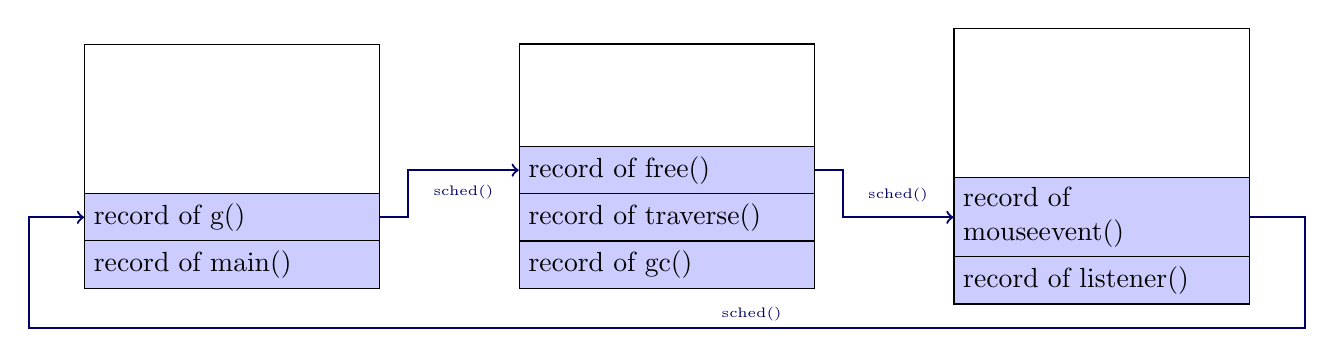
\begin{tikzpicture}
   [stack/.style={rectangle split, rectangle split parts=4,draw,
     text width=10em},
    scolor/.style={rectangle split part fill={white,blue!20!white,blue!20!white,blue!20!white}}]

\node [stack,scolor,rectangle split parts=3] (stk2) {
\nodepart{one} \rule{0pt}{4.7em}
\nodepart{two} record of g()
\nodepart{three} record of main()
};
\node [stack,scolor,right=5em of stk2] (stk1) {
\nodepart{one} \rule{0pt}{3em}
\nodepart{two} record of free()
\nodepart{three} record of traverse()
\nodepart{four} record of gc()
};
\node [stack,scolor, rectangle split parts=3,right=5em of stk1] (stk3) {
\nodepart{one} \rule{0pt}{4.7em}\hspace*{2em}
\nodepart{two} record of mouseevent()
\nodepart{three} record of listener()
};
\draw [->,blue!40!black,thick] (stk2.two east) -- +(1em,0) node [xshift=2em, yshift=.9em] {\fontsize{2}{2}\selectfont sched()} |- (stk1.two west);
\draw [->,blue!40!black,thick] (stk1.two east) -- +(1em,0) node [xshift=2em, yshift=-.9em] {\fontsize{2}{2}\selectfont sched()} |-  (stk3.two west);
\draw [->,blue!40!black,thick] (stk3.two east) -- +(2em,0) -- +(2em,-4em)  node [xshift=-20em, yshift=.5em] {\fontsize{2}{2}\selectfont sched()} -| ($(stk2.two west)+(-2em,0)$) --  (stk2.two west);
\end{tikzpicture}
}

\end{itemize}
\end{frame}
\end{document}
